\Tsubsection{UI2 Recolección y clasificación} 
%------------------------------------Objetivo----------------------------------%
\begin{large}
  \textbf{Objetivo}\\
\end{large}


Informar al usuario que la recolección y clasificación de noticias se está llevando acabo.\\

%------------------------------------Descripción---------------------------------%
\begin{large}
  \textbf{Descripción}\\
\end{large}

La Pantalla \ref{fig:UI2} muestra un mensaje flotante con la siguiente redacción: \textbf{En proceso de recolección y clasificación}, para informar al usuario que la consulta realizada está en proceso.\\

%-----------------------------------Salidas------------------------------------%
\begin{large}
  \textbf{Salidas}
\end{large}

\begin{itemize}

  \item Ninguno

\end{itemize}

%------------------------------------Comandos----------------------------------%


%------------------------------------Referencia----------------------------------%
\begin{large}
  \textbf{Referenciado por}
\end{large}

\begin{itemize}

  \item \Tref{CU1}{CU1 Recolectar noticias}

\end{itemize}  

%----------------------------------------Pantalla--------------------------------%


\begin{figure}\Tlabel{UI2}
  \centering 
	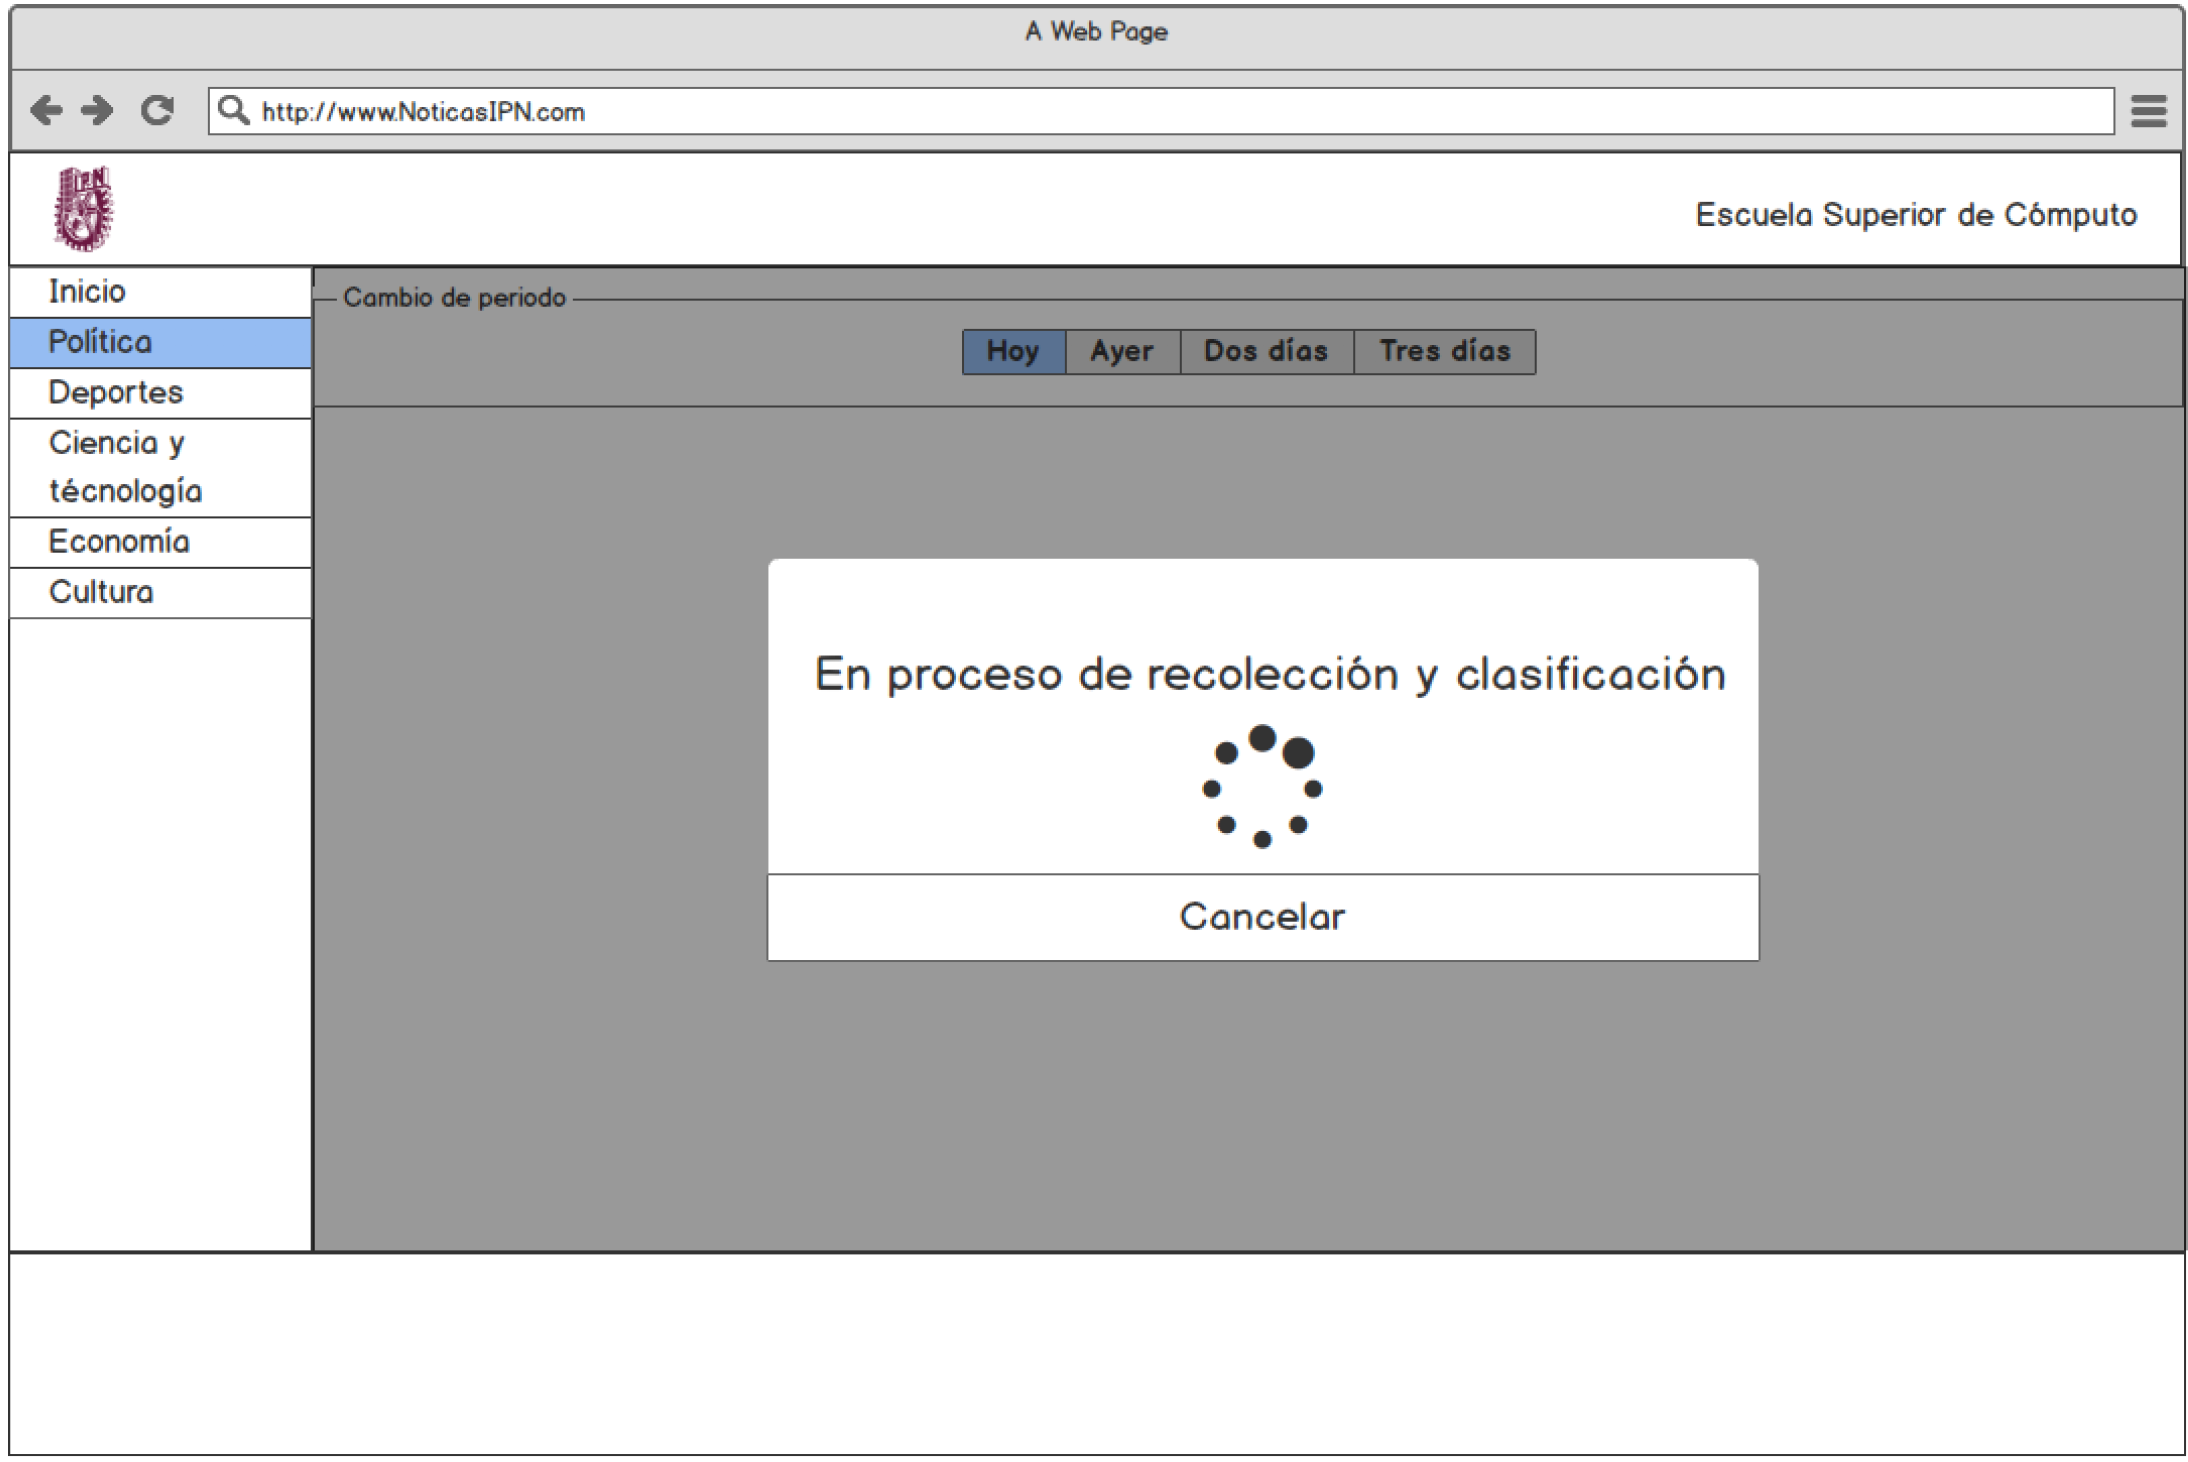
\includegraphics[scale=.32]{imagenes/Pantallas/UI2}
  \caption{Pantalla UI2 Espera de proceso}
  \label{fig:UI2}
\end{figure}
